\subsection{Формальные языки}

\deff{Алфавит} - $\Sigma$ - конечное или пустое

Множество слов длины $n$: $\Sigma^n$ 

$\Sigma^*=\bigcup\limits_{k=0}^\infty \Sigma^k$

\deff{Язык} - подмножество слов в алфавите $L \subset \Sigma^k$

\deff{Замечание.} Множество языков $2^{\Sigma^* }$ несчетно.

\subsection{Описание языка.}

Вот мы хотим описать язык. И описать его словами, например: все слова четной длины, они содержат четное число единиц. Но мы не можем дать эти слова компьютеру или человеку, говорящему на другом языке. 

Поэтому существует несколько способов описания языков:
\begin{enumerate}
    \item Перечисление: Явное перечисление всех слов в языке (возможно только для конечных языков). Например, $L = \{a, ab, aba\}$.
    \item Порождающая грамматика (формальная грамматика): Набор правил, определяющих, какие слова принадлежат языку.
    \item Распознающий автомат: Машина (например, конечный автомат), которая принимает или отклоняет слова в зависимости от того, принадлежат они языку или нет.
    \item Регулярное выражение: Шаблон, описывающий структуру слов в языке.
    \item  Предикат: Математическое условие, которому должны удовлетворять слова, чтобы принадлежать языку. 
\end{enumerate}

\textbf{Замечание.} Всего описаний счетное множество

\textbf{Фанфакт.} Если вы захотите найти лексикографически минимальный язык без описания, то когда вы найдете его, у него появится описание. Мы не будем думать об этом и такого рода парадоксах.

\subsection{Регулярные (автоматные языки)}

У нас есть операция конкатенации, определена она таким образом:

$\alpha, \beta \in \Sigma^*: \varphi = \alpha \beta$, причем $\alpha \in \Sigma^k, \beta \in \Sigma^l, \alpha\beta \in \Sigma^{k+l}$, а также $\varphi_i =\begin{cases}
    i \leq k \Rightarrow \alpha_i\\
    i > k \Rightarrow \beta_{i-k}
\end{cases}
$

Она ассоциативна, и есть нейтральный элемент $\varepsilon$.

Но теперь хотим ввести понятие \deff{конкатенации языков}:
$$AB = \{x \bigm| x = yz, y \in A,z \in B\}$$
\textbf{Пример:}

$A = \{0,01\}, B = \{0,10\}$, тогда $AB = \{00,010,0110\}$

А теперь обо всех операциях 

Пусть $L_1$ и $L_2$ - языки над алфавитом $\Sigma$. Тогда можно определить следующие базовые операции:
\begin{enumerate}
    \item Объединение: $L_1 \cup L_2 = \{w \bigm| w \in L_1\,\,  ||\,\, w \in L_2\}$
    \item  Конкатенация: $L_1 L_2 = \{w_1 w_2 \bigm| w_1 \in L_1, w_2 \in L_2\}$

    \item Степень: $L_1^0 = \{\varepsilon\},L_1^{n+1}=L_1L_1^n$

    \item Замыкание Клини: $A^* = \bigcup\limits_{k=0}^\infty A^k$
\end{enumerate}



$Reg_0 =\{\varnothing, \{\varepsilon\}, \{c\} \text{ for $c$ in $\Sigma$}\}$ - \deff{базовые регулярные языки}

$Reg_{i+1} = Reg_i \cup \{A\cup B,AB,A^* \bigm| A,B \in Reg_i\}$

\deff{Семейство регулярных языков:} $Reg = \bigcup\limits_{k=0}^\infty Reg_k$

\thmm{Лемма:} 

$A,B \in Reg \Rightarrow A \cup B \in Reg, AB \in Reg, A^* \in Reg$.

\textbf{Доказательство:}

$A \in Reg_i, B \in Reg_j,$ откуда по определению $A \cup B, AB, A^* \in Reg_{\max(i,j)+1}$.

\hfill Q.E.D.

$X\in Good, X \subset 2^{\Sigma^*}, X - \text{set$\langle$language$\rangle$}, Good  -\text{set$\langle$set$\langle $language$\rangle\rangle$}$ 

Good - множество множеств языков. Мы называем его \deff{хорошим} если:
\begin{enumerate}
    \item $Reg_0 \subset X$
    \item $X$ замкнут относительно базовых операций.
\end{enumerate}

\thmm{Теорема.} $Reg = \bigcap\limits_{u \in Good} u$

Доказательства не будет.

$\varnothing$ - пустое множество, $\varepsilon$ - пустая строка.

Пусть у языка $A$ описание $\alpha$. У языка $B$ описание $\beta$. Тогда введем обозначение:

\begin{enumerate}
    \item $AB$, описание будет $\alpha \beta$ --- средний приоритет
    \item $A \cup B$, описание будет $\alpha \bigm| \beta$ --- минимальный приоритет
    \item $A^*$, описание будет $a^*$ --- максимальный приоритет
\end{enumerate}

В зависимости от приоритета будем заключать выражения в скобки. Такие записи называются \deff{академическими регулярными выражениями}.

Также есть еще две обозначения:
\begin{enumerate}
    \item $\alpha^+  = \alpha \alpha^* $.
    \item $\alpha^k = \alpha\ldots \alpha$ - $k$ раз.
\end{enumerate}

\subsection{Детерминированный Конечный Автомат (ДКА)}

В разделе марковских цепей у нас были графы с вероятностями на ребрах. А давайте теперь удалим вероятности. 

$A = \langle \Sigma, Q,S,T, \delta: Q \times \Sigma \rightarrow Q \rangle$, где

\begin{enumerate}
    \item $\Sigma$ - алфавит
    \item $Q$ - конечное множество состояний
    \item $S\in Q$ - начальное состояние.
    \item $T\subset Q$ - допускающее (конечное) состояние. 
    \item $\delta$ - функция перехода, которая по текущему состоянию переходит
\end{enumerate}

$Snap = Q \times \Sigma^*$ --- \deff{множество мгновенных описаний} автомата или состояний.  $\vdash$ - операция перехода от одного описания к другому.

$\vdash: \langle q, \alpha \rangle \vdash \langle r,\beta\rangle$
\begin{enumerate}
    \item $\alpha = c\beta , c \in \Sigma$
    \item $r = \delta( q,c)$
\end{enumerate}

Это описание того, как мы бегаем по графу. То есть например пусть у нас есть автомат, который описывает четное или нечетное число единиц в строке, и ему подали $0101$. Тогда для него мгновенные описания:
$$\langle even, 0101\rangle \vdash \langle even, 101\rangle \vdash \langle odd, 01\rangle \vdash \langle odd , 1\rangle \vdash \langle even, \varepsilon\rangle$$
\deff{Язык автомата} $L(A) = \{w \bigm| \langle s,w\rangle \vdash^* \langle t, \varepsilon\rangle, t \in T\}$

\thmm{Теорема (Клини) } 

$Reg = Aut$, где $Aut$ - множество языков, задаваемых ДКА: $Aut = \{ X \bigm| \exists A: X = L(A)\}$, где $A$ --- ДКА.

Доказательства не будет

Пример ДКА:

\begin{center}
    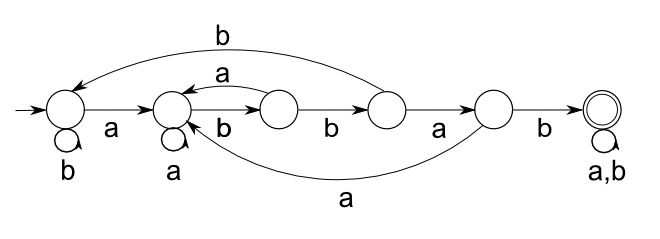
\includegraphics[width = 14cm]{assets/7_4_1.png}
\end{center}

Это автомат для поиска образца в тексте для строки "abbab".